\documentclass{beamer}

\setbeamertemplate{navigation symbols}{}
\setbeamertemplate{footline}[15]
\setbeamercolor{title}{fg=white,bg=darkred!80!black}
\usetheme{CambridgeUS}

\title[Protein fold classification]{Protein fold classification incorporating additional evolutionary information from phylogenetic profiles}
\author{Daniel S. Standage}
\date{\today}
\institute[BCB 569]{BCB 569}

\begin{document}
 

\begin{frame}
  \titlepage
\end{frame}

\section{Background}
\subsection{Protein science}
\begin{frame}
  \frametitle{Protein science}
  \begin{center}
    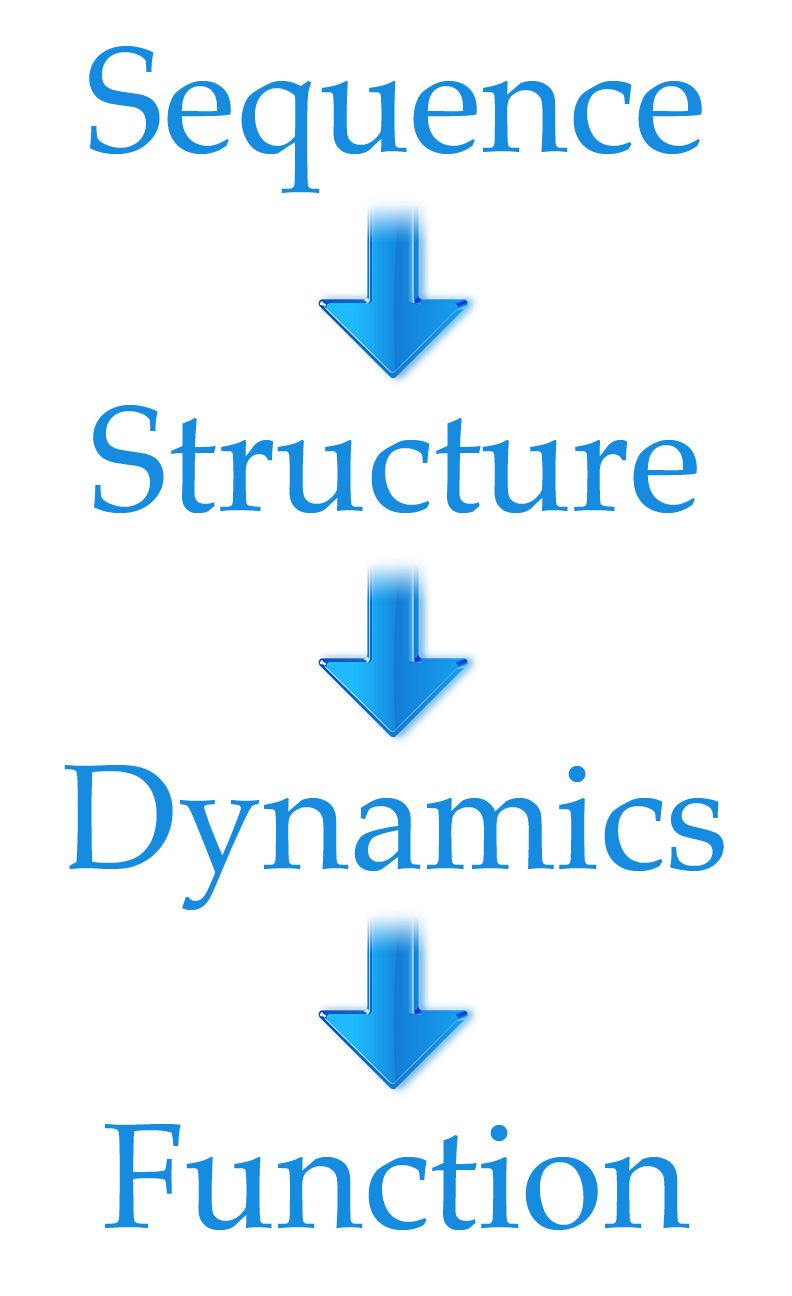
\includegraphics[width=125px]{paradigm.jpg}
  \end{center}
% Early on in this class, we discussed a central paradigm in protein science, the idea being that a protein sequence determines a protein structure, which determines protein dynamics, which determines protein function. Lots of sequences (protein sequencing, gene/transcript translations, computational predictions, etc), but determining structures (crystallography, NMR) is still difficult. Homology modeling can give good results, but sometimes no sequence homolog found: limitation.
\end{frame}
\begin{frame}
  \frametitle{Protein science}
  
  {\LARGE Homology modeling}
  \vspace{1px}
  \hrule
  \vspace{5px}
  \begin{itemize}
    \item ``sequence $\rightarrow$ structure" problem
    \item accurate when structure of a close homolog available
    \item need alternative that does not depend on sequence similarity
  \end{itemize}
\end{frame}

\subsection{Protein fold classification}
\begin{frame}
  \frametitle{Protein fold classification}
  \begin{center}
    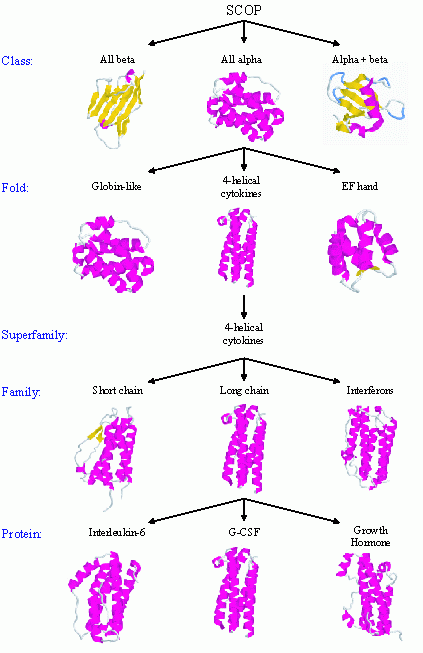
\includegraphics[width=125px]{scop-hier.png}
  \end{center}
\end{frame}
\begin{frame}
  \frametitle{Protein fold classification}
  \begin{center}
    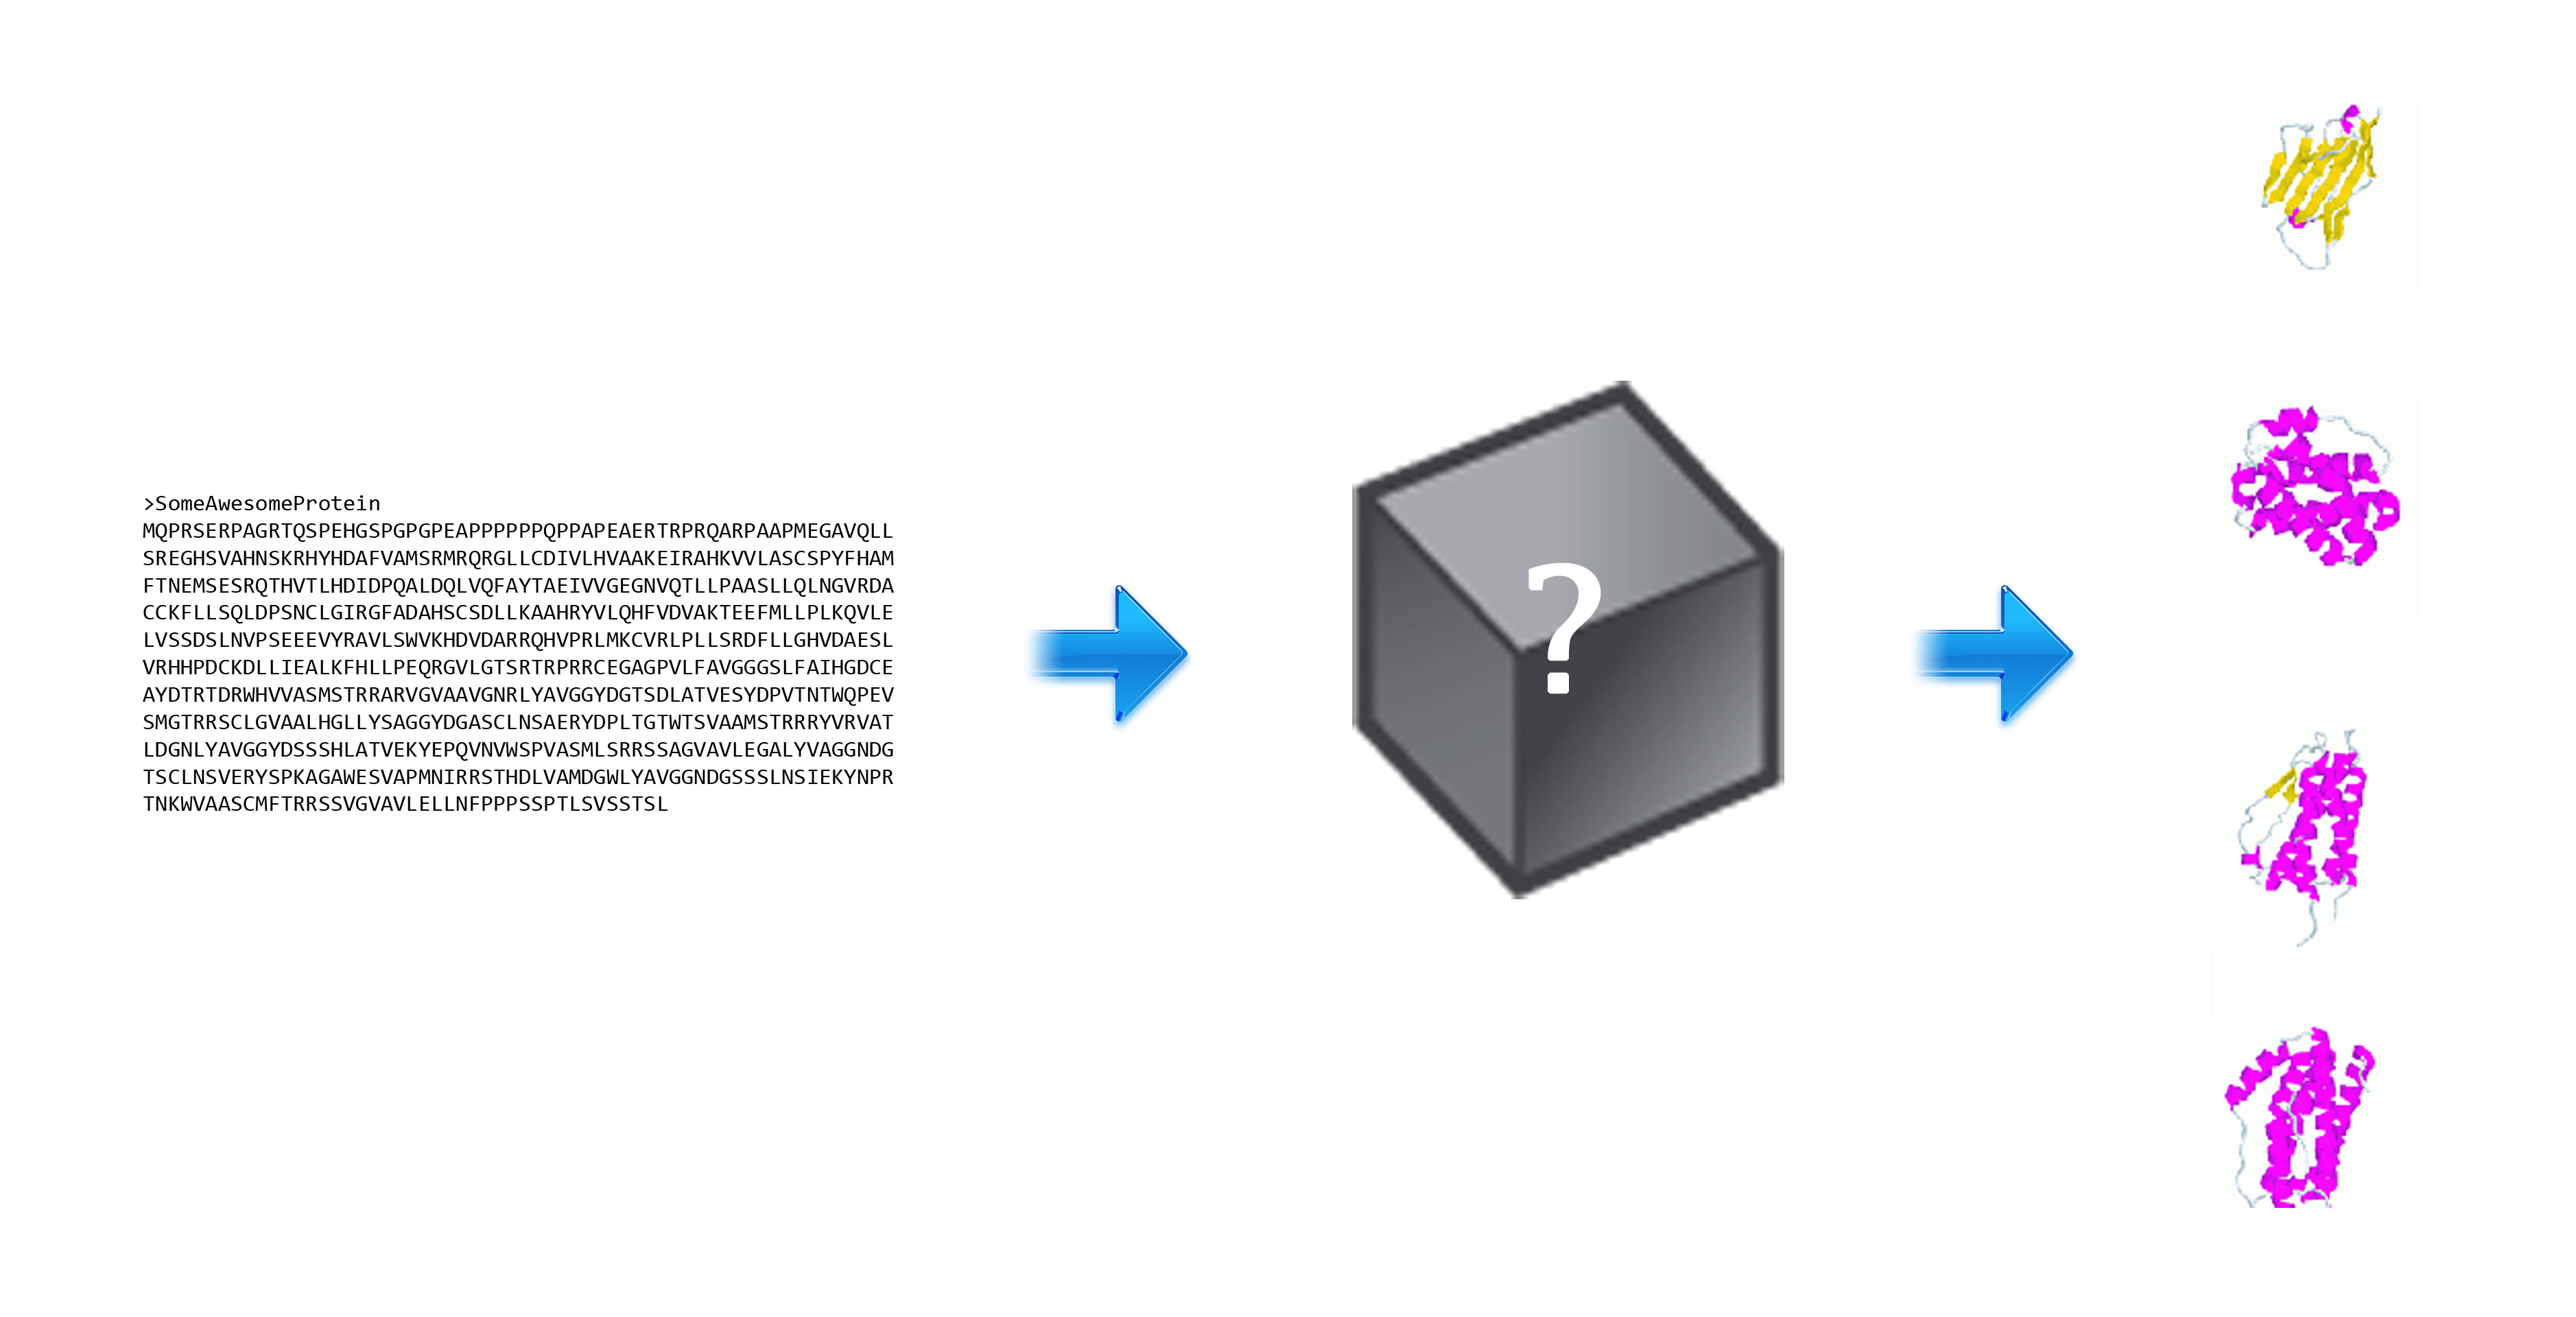
\includegraphics[width=325px]{classification-simple.jpg}
  \end{center}
\end{frame}
\begin{frame}
  \frametitle{Protein fold classification}
  {\LARGE My project}
  \vspace{1px}
  \hrule
  \vspace{5px}
  \begin{itemize}
    \item implement PFRES method
    \item extend method with new features
  \end{itemize}
\end{frame}


\section{Methods}

\subsection{Data}
\begin{frame}
  \frametitle{Data}
  
  \begin{itemize}
    \item includes sequences from 27 most populated folds in SCOP
    \item pairwise sequence similarity $< 35\%$
  \end{itemize}
  
\end{frame}
\begin{frame}
  \frametitle{Data}

  {\LARGE Training data}
  \vspace{1px}
  \hrule
  \vspace{5px}
  \begin{itemize}
    \item 313 domains (Ding \& Dubchak, 2001)
  \end{itemize}
  
  \vspace{30px}
  
  {\LARGE Testing data}
  \hrule
  \vspace{5px}
  \begin{itemize}
    \item 385 domains (Ding \& Dubchak, 2001)
    \item 908 domains (Shen \& Kurgan, 2007)
  \end{itemize}
\end{frame}

\subsection{Features}
\begin{frame}
  \frametitle{Features}
  \begin{center}
    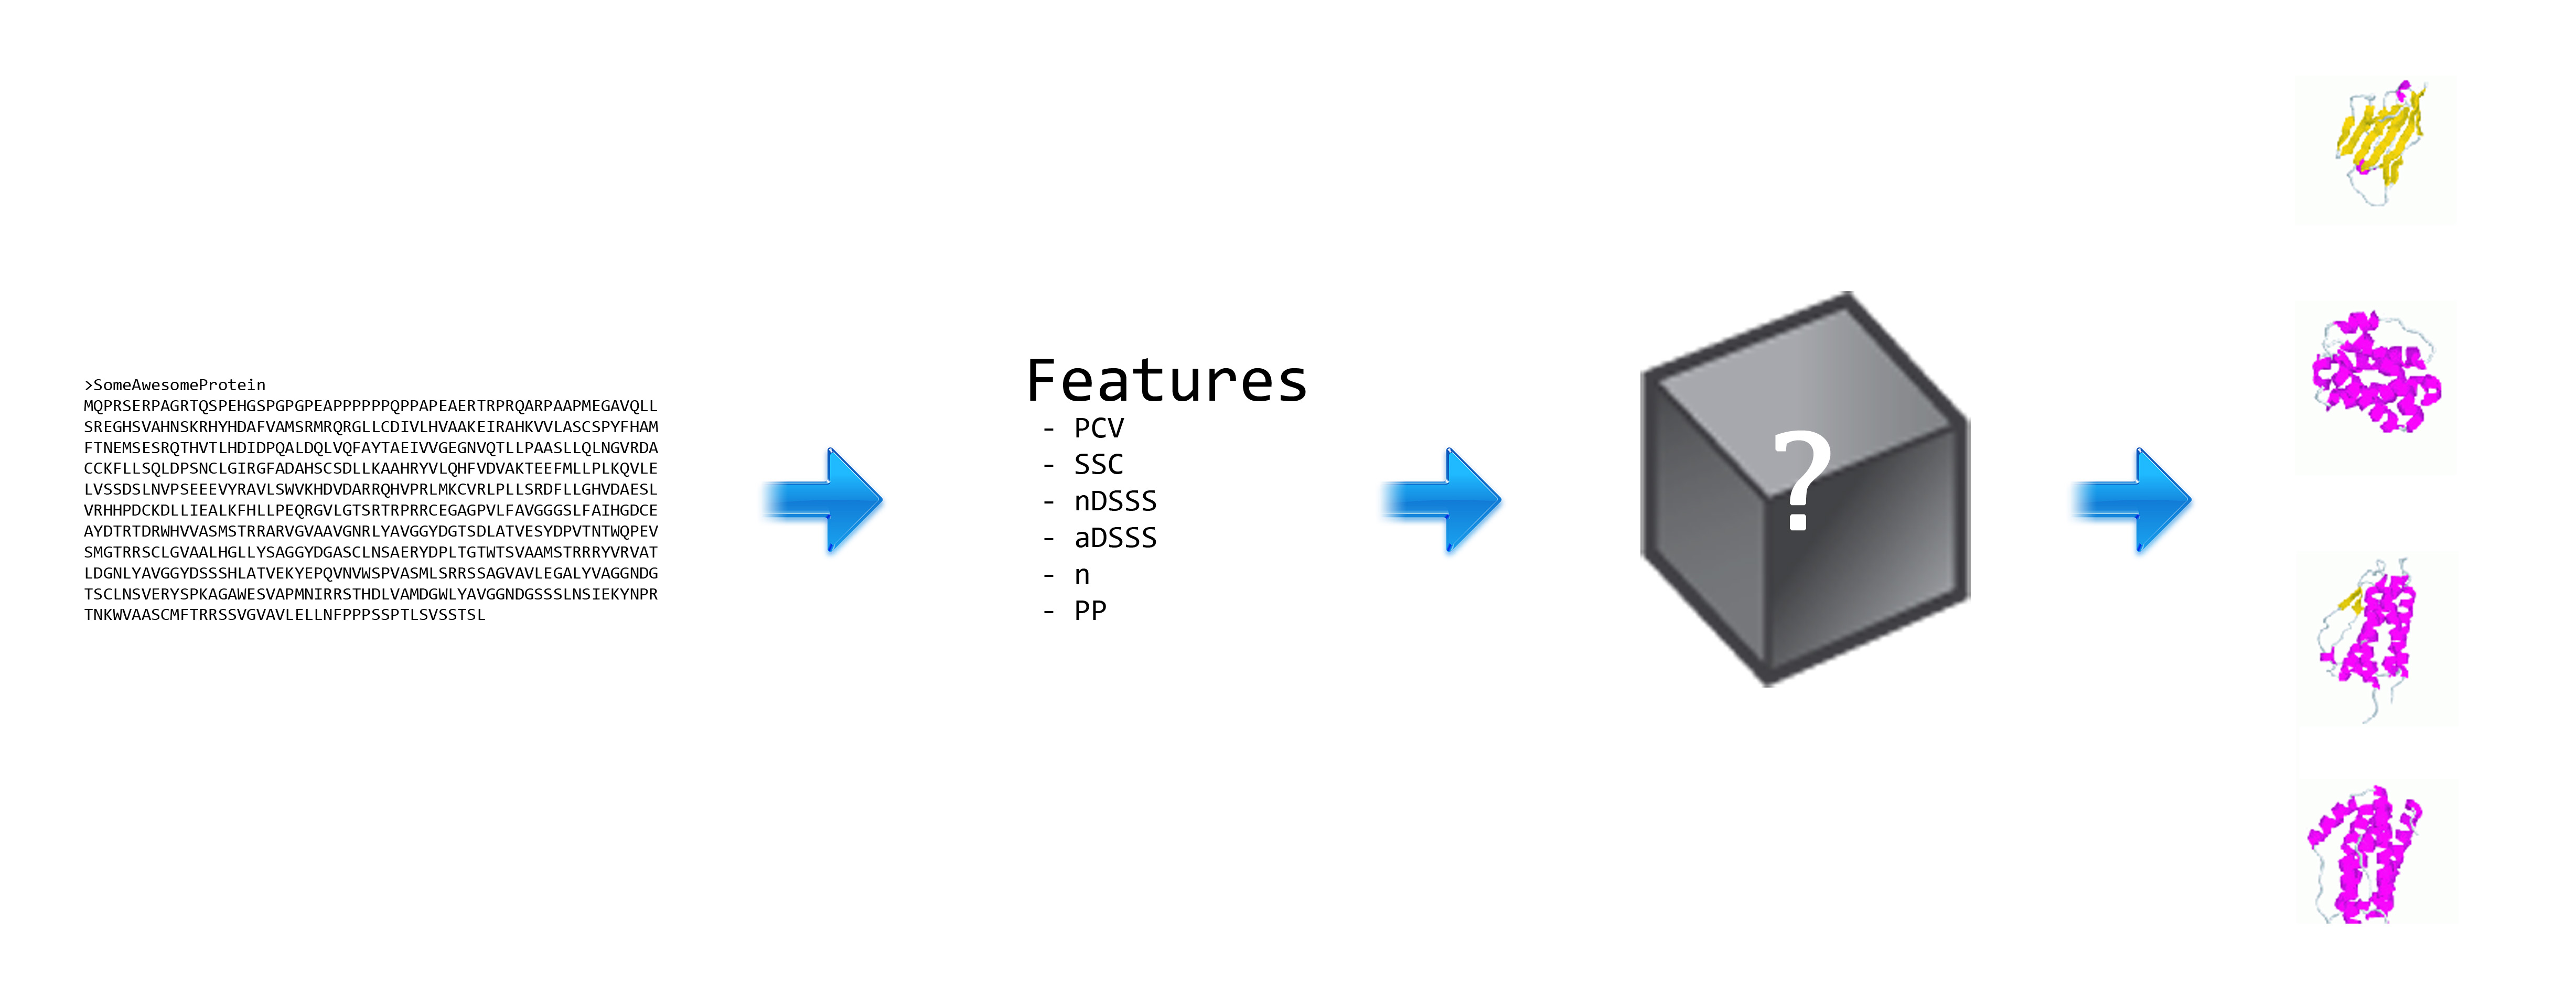
\includegraphics[width=325px]{classification.jpg}
  \end{center}
\end{frame}
\begin{frame}
  \frametitle{Profile-based composition vector (PCV)}
  \begin{itemize}
    \item search with PSI-BLAST
    \item generate PSSM $a_{ki}$ (an $L \times 20$ matrix)
    \item PCV has following form \[ PCV_i = \sum_{k=1}^{L}\frac{\max(a_{ki}, 0)}{L} \hspace{25px} (i=1,2,...,20) \]
  \end{itemize}
\end{frame}
\begin{frame}
  \frametitle{Profile-based composition vector (PCV)}
  \begin{table} \centering
  \begin{tabular}{ c | c c c c c } 
        & A & R & N & ... & Y \\ \hline
    1   & -3 & 1 & 2 & ... & 5 \\
    2   & -6 & 5 & -6 & ... & -2 \\
    ... & ... & ... & ... & ... & ... \\
    $L$ & 7 & 4 & 4 & ... & -3 \\
  \end{tabular}
  
  \vspace{25px}
  
  \[ PCV_i = \sum_{k=1}^{L}\frac{\max(a_{ki}, 0)}{L} \hspace{25px} (i=1,2,...,20) \]
  \vspace{5px}
\end{table}
\end{frame}
\begin{frame}
  \frametitle{Secondary-structure-based features}
  \begin{itemize}
    \item three structure categories: $H$=helix, $E$=strand, $C$=coil
    \item content: \textbf{SSC}
    \item contiguous segments: \textbf{DSSS}
    \item arrangements of contiguous segments: \textbf{ADSSS}
  \end{itemize}
\end{frame}
\begin{frame}
  \frametitle{Secondary-structure-based features}
  \begin{table} \centering
  \begin{tabular}{ l l } \hline
    $SSC_m$ & $m \in \{H, E, C\}$ \\
    $DSSS_m$ & $m \in \{H, E, C\}$ \\
    $ADSSS_{m}$ \hspace{15px} & $m \in \{H, E, C\}^{3}$ \\ \hline
  \end{tabular}
  \vspace{5px}
\end{table}
  \begin{center}
    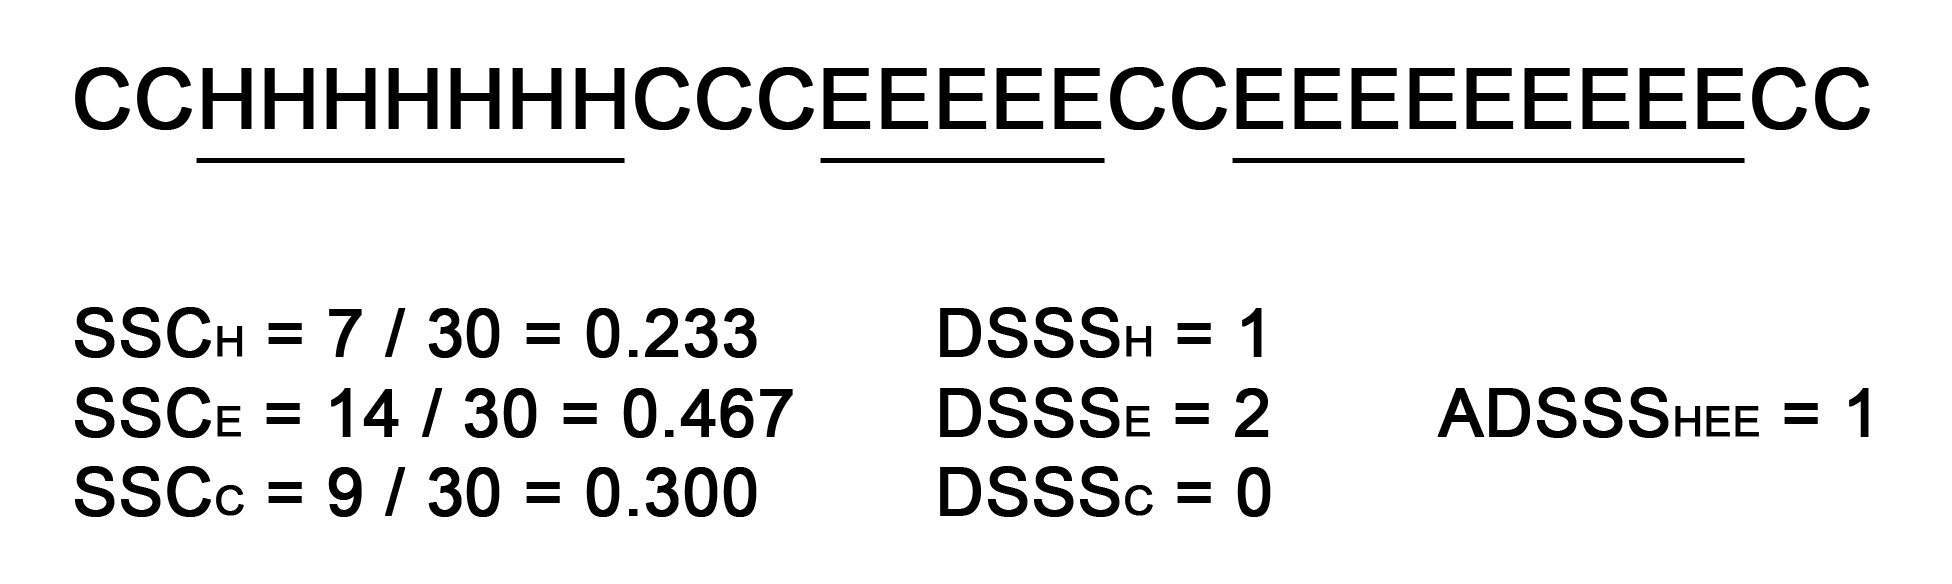
\includegraphics[width=325px]{../ss.png}
  \end{center}
\end{frame}
\begin{frame}
  \frametitle{Phylogenetic profile}
  \begin{itemize}
    \item captures phylogenetic distribution of protein
    \item database of $n$ reference genomes $G = \{ G_1, G_2, ..., G_n \}$
    \item phylogenetic profile of a gene $g$ \[ p = p_1 p_2 ... p_n \hspace{10px}\text{s.t.}\hspace{10px} p_i = 1 \hspace{10px}\text{if}\hspace{10px} g \in G_i \]
  \end{itemize}
\end{frame}
\begin{frame}
  \frametitle{Full feature space}
  \begin{table} \centering
  \begin{tabular}{ l l }
    \hline
    \multicolumn{1}{c}{\textbf{Characteristic}} & \textbf{\# Features} \\ \hline
    PCV    & 20 \\
    SSC    & 3  \\
    DSSS   & 3  \\
    ADSSS  & 27 \\
    Length & 1  \\
    Phylogenetic profile \hspace{15px} & 12 \\
    \textbf{Total} & \textbf{66} \\ \hline
  \end{tabular}
  \vspace{5px}
\end{table}
\end{frame}
\begin{frame}
  \frametitle{Feature calculation}
  \begin{itemize}
    \item PCVs
      \begin{itemize}
        \item PSI-BLAST
        \item NR database
      \end{itemize}
    \item SS features
      \begin{itemize}
        \item PSI-PRED
        \item Uniref90 database
      \end{itemize}
    \item phylogenetic profiles
      \begin{itemize}
        \item new code
        \item custom protein databases
      \end{itemize}
    \item parallel pipeline
  \end{itemize}
\end{frame}


\begin{frame}
  \frametitle{Phylogenetic profile}
\begin{table} \centering
  \begin{tabular}{ l l }
    \hline
    \multicolumn{1}{c}{\textbf{Eukaryotes}} & \multicolumn{1}{c}{\textbf{Dicots}} \\ \hline
    \textit{Arabidopsis thaliana} & \textit{Arabidopsis thaliana} \\
    \textit{Aspergillus nidulans} & \textit{Carica papaya} \\
    \textit{Cryptosporidium parvum} & \textit{Cucumis sativus} \\
    \textit{Danio rerio} & \textit{Glycine max} \\
    \textit{Drosophila melanogaster} \hspace{15px} & \textit{Lotus japonicus} \\
    \textit{Eremothecium gossypii} & \textit{Manihot esculenta} \\
    \textit{Homo sapiens} & \textit{Medicago trunculata} \\
    \textit{Mus musculus} & \textit{Mimulus guttatus} \\
    \textit{Physcomitrella patens} & \textit{Populus trichocarpa} \\
    \textit{Plasmodium falciparum} & \textit{Prunus persica} \\
    \textit{Saccharomyces cerevisiae} & \textit{Ricinus communis} \\
    \textit{Zea mays} & \textit{Solanum lycoparsicum} \\ \hline
  \end{tabular}
  \vspace{5px}
\end{table}
\end{frame}
\begin{frame}
  \frametitle{Data set feature spaces}
  \begin{table} \centering
  \begin{tabular}{ c c c c }
    \hspace{10px} & \textbf{Training Set} & \textbf{Test Set 1} & \textbf{Test Set 2} \\ \hline
    \textbf{PFRES}        & $Tr_{P}$ & $T1_{P}$ & $T2_{P}$ \\
    \textbf{PFRES + Euk.} & $Tr_{PE}$ & $T1_{PE}$ & $T2_{PE}$ \\
    \textbf{PFRES + Dic.} & $Tr_{PD}$ & $T1_{PD}$ & $T2_{PD}$ \\ \hline
  \end{tabular}
  \vspace{5px}
\end{table}
\end{frame}
\begin{frame}
  \frametitle{Feature selection: information gain}
  \begin{table} \centering
  \begin{tabular}{ l l l }
    \hline
    \multicolumn{1}{c}{\textbf{Characteristic}} & \textbf{\# Features} & \multicolumn{1}{c}{\textbf{Selected Features}} \\ \hline
    PCV    & 20 & 20 \\
    SSC    & 3  & 3 \\
    DSSS   & 3  & 3 \\
    ADSSS  & 27 & 10 \\
    Length & 1 & 1 \\
    Phylogenetic profile & 12 & 6 \\
    \textbf{Total} & \textbf{66} & \textbf{43} \\ \hline
  \end{tabular}
  \vspace{5px}
\end{table}
\end{frame}

\subsection{Machine learning}
\begin{frame}
  \frametitle{Machine learning}
  \begin{center}
    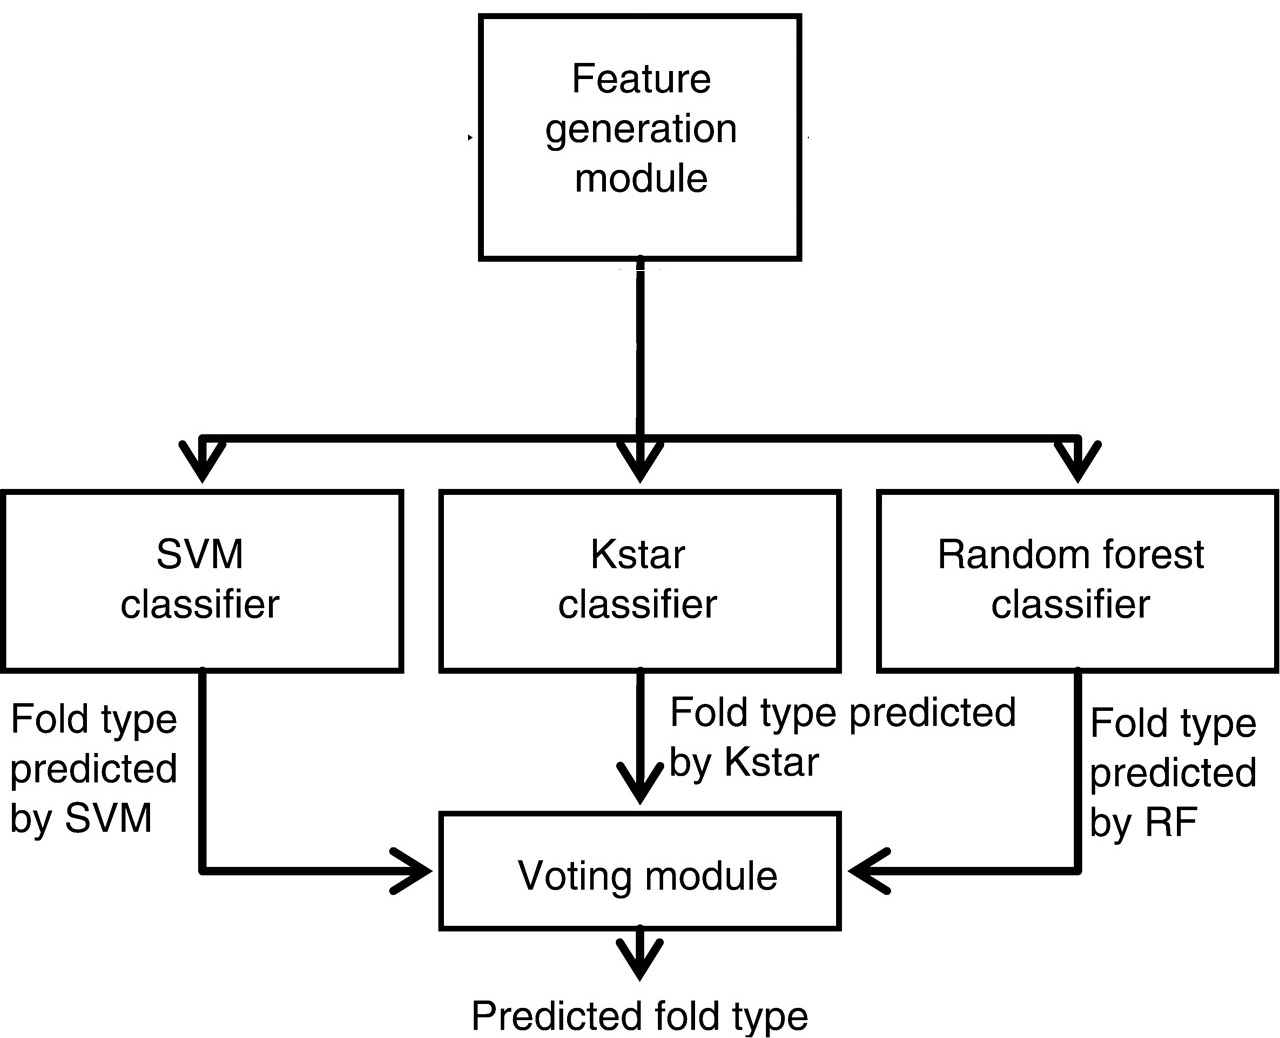
\includegraphics[width=225px]{pfres.jpg}
  \end{center}  
\end{frame}
\begin{frame}
  \frametitle{Machine learning}
  \begin{center}
    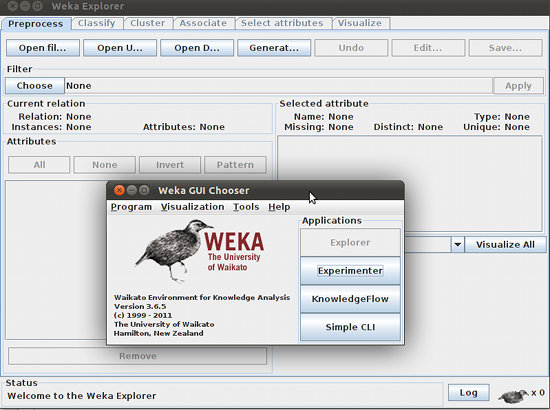
\includegraphics[width=225px]{weka.png}
  \end{center}  
\end{frame}

\subsection{Results}
\begin{frame}
  \frametitle{Results}
  \begin{table} \centering
  \begin{tabular}{ c c c c c }
    \hline
    \textbf{Classifier} & \textbf{Eukaryotes} & \textbf{Dicots} & \textbf{PFRES} & \textbf{Published} \\ \hline
    \multicolumn{1}{l}{RF} & \multicolumn{4}{c}{\hspace{15px}} \\
    \multicolumn{1}{r}{Test 1} & \textbf{65.8\%} & 62.9\% & 65.5\% & 66.8\% \\
    \multicolumn{1}{r}{Test 2} & \textbf{64.6\%} & 59.8\% & 64.0\% & 63.3\% \\
    \multicolumn{1}{l}{SVM} & \multicolumn{4}{c}{\hspace{15px}} \\
    \multicolumn{1}{r}{Test 1} & 61.4\% & 54.8\% & 66.8\% & 66.1\% \\
    \multicolumn{1}{r}{Test 2} & 53.1\% & 51.1\% & 62.9\% & 62.4\% \\
    \multicolumn{1}{l}{Kstar} & \multicolumn{4}{c}{\hspace{15px}} \\
    \multicolumn{1}{r}{Test 1} & \textbf{63.2\%} & 57.2\% & 63.2\% & 65.0\% \\
    \multicolumn{1}{r}{Test 2} & \textbf{59.4\%} & 52.5\% & 56.7\% & 62.7\% \\
    \multicolumn{1}{l}{Ensemble \hspace{25px} ~} & \multicolumn{4}{c}{\hspace{15px}} \\
    \multicolumn{1}{r}{Test 1} & 65.8\% & 60.1\% & 67.1\% & 68.4\% \\
    \multicolumn{1}{r}{Test 2} & \textbf{62.7\%} & 56.5\% & 62.6\% & 66.4\% \\ \hline
  \end{tabular}
  \vspace{5px}
\end{table}
\end{frame}

\subsection{Conclusions}
\begin{frame}
  \frametitle{Conclusions}
  \begin{itemize}
    \item Short phylogenetic profiles do not provide a significant performance improvement.
    \item My method performed comparably despite the higher-dimensional feature space.
    \item With more training data and longer phylogenetic profiles, I expect a substantial performance improvement.
  \end{itemize}
\end{frame}

\subsection{Acknowlegements}
\begin{frame}
  \frametitle{Acknowlegements}
  \begin{itemize}
    \item Dr. Jernigan
    \item Dr. Hongbin Shen
    \item Dr. Lukasz Kurgan
  \end{itemize}
\end{frame}

\subsection{Acknowlegements}
\begin{frame}
  \frametitle{Acknowlegements}
  \begin{center}
  {\LARGE Thank you!}
  \vspace{5px}
  \end{center}
\end{frame}

\end{document}
